\documentclass{article}
\usepackage{amsmath}
\usepackage{amssymb}
\usepackage{graphicx}
\usepackage{authblk}
\usepackage{hyperref}
\usepackage[margin=1in]{geometry}
\usepackage{tikz}
\usetikzlibrary{positioning}


\title{A Layered Epistemic Algorithm for Reliability-Weighted Inference in Spatial and Multimodal Intelligence}
\author{Joe Yap}
\affil{Independent Researcher}
\date{12/9/2025}

\begin{document}

\maketitle

\begin{abstract}
Spatial and embodied intelligence require not only accurate perception but also principled strategies for interpreting mismatches between observation and expectation. This note introduces a \textbf{Layered Epistemic Algorithm}, a simple but general rule for anomaly handling in intelligent systems. The Algorithm states that belief updates should scale with the reliability of the information channel and the surprise of the observation, and further that inconsistencies should be interpreted in a fixed causal order: channel before assumptions before model. This framework complements multimodal AI, robotics, grounded cognition, and world-model learning by providing a unified reliability-weighted mechanism for belief revision.
\end{abstract}

\section{Introduction}

Intelligent agents operating in uncertain environments must continuously interpret incoming observations and determine how strongly these observations should influence their internal beliefs. Even in structured reasoning tasks, localized inconsistencies arise frequently due to noise, occlusion, environmental conditions, or incomplete assumptions. Without principled anomaly handling, an agent may overreact to noise, underreact to genuine anomalies, or prematurely revise its core model.

We propose a \textbf{Layered Epistemic Algorithm} that formalizes how agents should weight evidence, interpret inconsistencies, and update beliefs. The Algorithm is broadly applicable to spatial intelligence, multimodal reasoning, robotics, and cognitive-style world-models. It is intentionally presented as a conceptual principle rather than a fully specified algorithm, with the goal of providing a compact, cross-domain rule for robust anomaly interpretation.

\section{Relation to Existing Epistemic and Bayesian Frameworks}

Although the mathematical components of this Algorithm draw on familiar Bayesian concepts such as likelihood, reliability weighting, and prediction error, the Algorithm itself is not a restatement of standard Bayesian inference. The contribution here is a \emph{new epistemic rule}: a structured, three-layer ordering for interpreting inconsistencies (channel $\rightarrow$ assumptions $\rightarrow$ model), imposed as an explicit priors-over-causes principle rather than being left implicit in a generative model. Traditional Bayesian formulations treat all explanatory hypotheses within a single unified inference step, whereas the proposed Algorithm elevates the diagnostic ordering itself to a first-class design constraint. This layered structure is conceptually new and aims to guide robust reasoning in multimodal and embodied settings where channels, assumptions, and world-models fail in qualitatively different ways.

\section{Example: Anomaly Interpretation in Structured Reasoning}

Consider a structured reasoning scenario in which values propagate through a diagram, and the agent infers a governing rule. Most intermediate values follow a consistent pattern, yet a single outlier appears. The agent must determine whether this discrepancy reflects:
\begin{itemize}
    \item a misread or unreliable input channel,
    \item an unstated contextual assumption,
    \item or a flaw in the inferred rule.
\end{itemize}

Different epistemic policies produce different reasoning behaviors. A pattern-first heuristic may discount the anomaly as noise; a reliability-aware policy treats the anomaly as high-value evidence. This discrepancy motivates a structured, layered interpretation of anomalies.

\section{Epistemic Phase Change}

A notable phenomenon occurs when shifting epistemic policies: a small adjustment in how anomalies are prioritized can yield a qualitative shift in the inferred model structure. Under default heuristics, a surprising observation may be ignored or explained away locally. Under the proposed Algorithm, the same observation---if it is both reliable and surprising---triggers a search for a globally coherent explanation.

This \textbf{epistemic phase change} illustrates how meta-level reasoning rules affect inference quality. Such transitions are central to robust AI reasoning, whether in spatial perception, multimodal fusion, or grounded world-modeling.

\section{The Layered Epistemic Algorithm}

Let:
\begin{itemize}
    \item $o$ be an observation,
    \item $C$ be the channel producing $o$,
    \item $r(C) \in [0,1]$ be the reliability of $C$,
    \item $M$ be the agent's current model,
    \item $A$ be auxiliary assumptions or environmental context.
\end{itemize}

\subsection{Core Update Rule}

The magnitude of the belief update is given schematically by
\begin{equation}
\Delta \text{Belief} \propto r(C) \cdot \text{Surprise}(o \mid M, A),
\end{equation}
where $\text{Surprise}(o \mid M, A)$ measures the prediction error relative to the agent's expectations under $M$ and $A$.

Intuitively, belief change should be greatest when an observation is \emph{both} highly reliable and highly surprising under the current model and assumptions. Conversely, low-reliability or low-surprise observations should produce small updates.

\subsection{Operationalizing $r(C)$ and Surprise}

The quantities $r(C)$ and $\text{Surprise}(o \mid M, A)$ are intentionally defined at the level of an epistemic principle rather than a fixed algorithmic prescription. In practice, $r(C)$ may be instantiated as any measure of channel reliability, including inverse sensor noise variance in robotics, confidence scores in vision systems, or uncertainty estimates derived from model ensembles or calibration techniques. Likewise, $\text{Surprise}(o \mid M, A)$ may be implemented as negative log-likelihood under a predictive model, as a prediction-error norm, or as a divergence between expected and observed features. The Algorithm does not depend on a specific functional form; rather, it asserts that belief updates should scale with whichever reliability and surprise estimates are appropriate for the system. This flexibility allows the Algorithm to apply uniformly across perceptual modalities, symbolic reasoning tasks, and multimodal architectures.

The use of a scalar reliability term $r(C)$ is a deliberate simplification at the level of the Algorithm. In real systems, uncertainty is often multidimensional, state-dependent, or represented by full covariance structures rather than a single number. Nothing in the Algorithm precludes such richer forms; $r(C)$ may be replaced by a vector of reliability components, a covariance matrix, or a learned uncertainty estimate without altering the principle itself. The scalar formulation serves only to express the epistemic role of channel reliability in the simplest possible form. As empirical implementations of the Algorithm mature, more expressive representations of reliability can be employed where appropriate, but the conceptual structure---the scaling of belief updates by channel trustworthiness---remains unchanged.

A full operational instantiation of $r(C)$ and $\text{Surprise}(o \mid M, A)$ is left to future work. Here we focus on establishing the conceptual framework. Once the epistemic structure is validated, subsequent work can formalize specific computational realizations appropriate to different modalities and architectures.

\subsection{Layered Hypothesis Ordering}

When $o$ contradicts the predictions of $M$ under assumptions $A$, the agent evaluates three classes of hypotheses:
\begin{itemize}
    \item $H_0$: channel or context error,
    \item $H_1$: auxiliary assumption error,
    \item $H_2$: core model error.
\end{itemize}

We impose the prior ordering
\begin{equation}
P(H_0) \ge P(H_1) \ge P(H_2),
\end{equation}
and a diagnostic sequence
\begin{equation}
H_0 \rightarrow H_1 \rightarrow H_2.
\end{equation}

Distinguishing between the hypotheses $H_0$, $H_1$, and $H_2$ is governed by the prior structure of the Algorithm rather than by a single inference step. The key insight is that different layers fail with vastly different frequencies in real systems. Physical laws and stable model structures typically have extremely high prior confidence, whereas observations and situational assumptions fail far more often. Thus, when an inconsistency arises, it is overwhelmingly more plausible that the observation channel is degraded or an assumption is violated than that the underlying model itself has changed. This mirrors scientific practice: anomalous readings are first attributed to instrumentation or context before concluding that new physics is required. The Algorithm formalizes this reasoning pattern by imposing a structured diagnostic ordering---channel $\rightarrow$ assumptions $\rightarrow$ model---which serves as an epistemic prior rather than a commitment to any specific algorithmic test. Systems may still evaluate multiple explanations, but the Algorithm encodes the relative plausibility of each layer as the guiding heuristic.

Although the diagnostic ordering $H_0 \rightarrow H_1 \rightarrow H_2$ provides a structured prior over explanatory causes, the Algorithm does not require that anomalies originate from a single layer. Real systems often experience mixed failures---for example, partial channel degradation combined with incorrect contextual assumptions. The Algorithm is compatible with such cases: the agent may maintain nonzero belief mass across multiple hypotheses and progressively reduce or refine them as additional evidence becomes available. This is analogous to existing reasoning and inference processes in probabilistic models, where explanations are iteratively narrowed rather than decided in a single step. The layered ordering therefore functions not as an exclusivity constraint, but as a principled guide for the order in which explanations should be examined and eliminated during convergence toward a coherent interpretation.

\section{Diagram: Layered Anomaly Interpretation}

\begin{verbatim}
                  Observation (o)
                         |
                         v
                  +----------------+
                  |   r(C)        |
                  | Reliability   |
                  +----------------+
                         |
                         v
                Surprise(o | M, A)
                         |
                         v
           +--------------------------------+
           |   Layered Hypothesis Ladder    |
           |--------------------------------|
           |  H0: Channel / Context Error   |
           |  H1: Assumption Error          |
           |  H2: Core Model Error          |
           +--------------------------------+
                         |
                         v
                   Belief Update
        ΔBelief ∝ r(C) × Surprise(o | M, A)
\end{verbatim}


\subsection{Case Study: The Yoshigahara Phase Change}

This example is adapted from a numeric tree puzzle attributed to Nob Yoshigahara, a noted Japanese puzzle designer whose works often require abandoning an initially plausible local rule in favor of a deeper global structure.

Consider a numeric tree in which each parent node is assumed to be determined by a simple arithmetic relationship between its two children. A natural first hypothesis is the \emph{subtraction model}, under which each parent equals the absolute difference of its children. This model fits the upper portion of the tree exactly: for instance,
\(|99 - 72| = 27\), \(|45 - 27| = 18\), and \(|39 - 18| = 21\).

A discrepancy emerges at a lower node with children \(13\) and \(21\). The subtraction model predicts a parent value of \(8\), yet the observed value is \(7\). This mismatch produces high surprise under the current model.

Two epistemic policies produce qualitatively different inferences:

\paragraph{Low-Reliability Interpretation (Favoring \(H_0\)).}
If the observation is assumed to come from a noisy or unreliable channel, the agent attributes the mismatch to a channel error (\(H_0\)). The value ``7'' is treated as a likely transcription mistake, the subtraction model is retained, and the remaining unknown in the puzzle is inferred consistently with that model.

\paragraph{High-Reliability Interpretation (Favoring \(H_2\)).}
If the observation is instead assumed to be highly reliable---as is appropriate for a carefully designed logic puzzle---the gate for \(H_0\) effectively closes. The anomaly then forces evaluation of deeper hypotheses, and the agent concludes that the subtraction model itself must be incorrect (\(H_2\)). A search for an alternative rule yields a relationship consistent with all nodes, including the anomalous one.

\paragraph{Epistemic Phase Change.}
The two interpretations differ not in the data but in the epistemic policy governing whether the anomaly activates \(H_0\) or \(H_2\). A small change in channel reliability \(r(C)\) induces a qualitative shift in reasoning: from treating the anomaly as noise to treating it as decisive evidence for model revision. This illustrates how the Layered Epistemic Algorithm governs the flow of inference and how the ordering \(H_0 \rightarrow H_1 \rightarrow H_2\) shapes an agent's willingness to abandon an initially adequate model in favor of a more globally coherent one.

% put these in your preamble if not already there
\usepackage{tikz}
\usetikzlibrary{positioning}

% ... later, where you want the figure:
\begin{figure}[h]
\centering

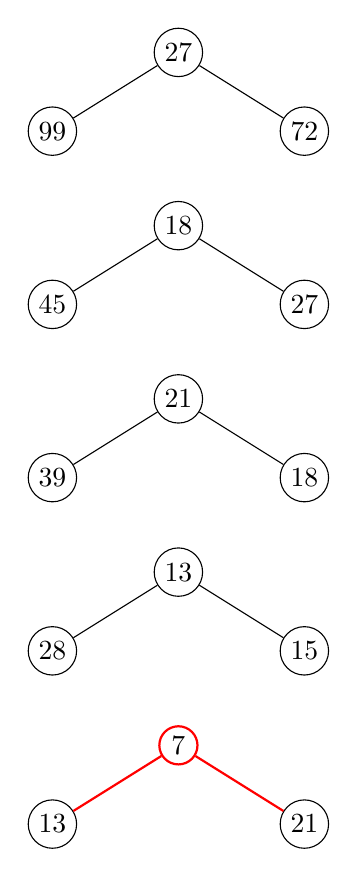
\begin{tikzpicture}[node/.style={circle, draw, inner sep=2pt}]
  % Row 1: 99, 72 -> 27
  \node[node] (r1p) at (0,0) {27};
  \node[node] (r1l) at (-1.6,-1) {99};
  \node[node] (r1r) at ( 1.6,-1) {72};
  \draw (r1p) -- (r1l);
  \draw (r1p) -- (r1r);

  % Row 2: 45, 27 -> 18
  \node[node] (r2p) at (0,-2.2) {18};
  \node[node] (r2l) at (-1.6,-3.2) {45};
  \node[node] (r2r) at ( 1.6,-3.2) {27};
  \draw (r2p) -- (r2l);
  \draw (r2p) -- (r2r);

  % Row 3: 39, 18 -> 21
  \node[node] (r3p) at (0,-4.4) {21};
  \node[node] (r3l) at (-1.6,-5.4) {39};
  \node[node] (r3r) at ( 1.6,-5.4) {18};
  \draw (r3p) -- (r3l);
  \draw (r3p) -- (r3r);

  % Row 4: 28, 15 -> 13
  \node[node] (r4p) at (0,-6.6) {13};
  \node[node] (r4l) at (-1.6,-7.6) {28};
  \node[node] (r4r) at ( 1.6,-7.6) {15};
  \draw (r4p) -- (r4l);
  \draw (r4p) -- (r4r);

  % Row 5: 13, 21 -> 7  (anomaly)
  \node[node, draw=red, thick] (r5p) at (0,-8.8) {7};
  \node[node]                    (r5l) at (-1.6,-9.8) {13};
  \node[node]                    (r5r) at ( 1.6,-9.8) {21};
  \draw[red, thick] (r5p) -- (r5l);
  \draw[red, thick] (r5p) -- (r5r);
\end{tikzpicture}
\caption{Numeric relations in the Yoshigahara puzzle. 
Each row shows two children and their parent. The subtraction rule 
$|a-b|=c$ fits the first four rows but fails for the last, where 
$|21-13|=8$ instead of the observed $7$, creating the anomaly that 
triggers the epistemic phase change.}
\end{figure}



\section{Relevance to Spatial and Embodied Intelligence}

Spatial intelligence depends on high-reliability perceptual channels that define objects, geometry, and affordances. The proposed Algorithm integrates naturally with such systems by weighting evidence appropriately and providing a formal mechanism for handling inconsistent observations.

Embodied agents frequently encounter noise, occlusion, and shifting context. The Algorithm offers a general-purpose reliability framework that bridges perception and reasoning, supporting the full loop:
\[
\text{Perceive} \rightarrow \text{Interpret} \rightarrow \text{Resolve Inconsistency} \rightarrow \text{Update Model} \rightarrow \text{Perceive Again}.
\]
In multimodal agents, where visual, proprioceptive, linguistic, and other signals must be integrated, the layered treatment of anomalies provides a uniform way to decide whether to distrust a channel, revise a contextual assumption, or reconsider a global world-model.

\section{Illustrative Examples and Future Empirical Work}

Although this note does not include a full empirical evaluation, the Algorithm lends itself naturally to simple illustrative examples, which we leave to future work once the conceptual framework is established. A typical demonstration would involve two observation channels with differing reliabilities and a single anomalous data point: under the Algorithm, a high-reliability, high-surprise anomaly would trigger a structured diagnostic search (channel $\rightarrow$ assumptions $\rightarrow$ model), whereas a low-reliability anomaly would be discounted. Similar thought experiments can be constructed for multimodal perception or diagram-based reasoning tasks. These examples are straightforward to instantiate, but the present work focuses on articulating the underlying epistemic principle; empirical illustrations will follow once the foundational structure is validated.

\section{Epistemic Scope and Relationship to Action}

The proposed Algorithm is explicitly epistemic: it governs how an agent updates its internal beliefs in response to anomalous observations, and it does not prescribe a decision-making or control strategy. Any downstream planning or action-selection mechanism---whether based on reinforcement learning, optimal control, active inference, or heuristic policies---can operate on the beliefs updated by this Algorithm. In addition to serving as a foundation for belief revision, the Algorithm also provides a principled criterion for \emph{when} to continue a reasoning chain and when to halt or redirect it: high-reliability, high-surprise observations warrant deeper inference, whereas low-reliability signals justify interrupting or discounting further reasoning. Thus, while the Algorithm does not define a full behavioural policy, it naturally interfaces with decision frameworks by modulating the flow of reasoning itself. Integrating this epistemic rule with specific action models remains an important direction for future work but lies outside the scope of the present note.

\section{Scope and Limitations}

The Layered Epistemic Algorithm is intended as a conceptual principle for belief revision and anomaly interpretation, not as a complete inference or control framework. It assumes that the agent maintains a predictive model $M$, a set of auxiliary assumptions $A$, and some means of estimating channel reliability $r(C)$, but it does not prescribe how these components are learned or represented. The Algorithm does not address adversarial settings, strategic manipulation, or environments where the generative structure is unknown or undefined. Its role is to guide epistemic organization---how explanations are prioritized and how belief updates are weighted---while leaving the design of decision policies, uncertainty estimators, and learning mechanisms to domain-specific methods. As such, the Algorithm should be viewed as a foundational reasoning principle that complements, rather than replaces, existing computational frameworks.

\section{Conclusion}

The Layered Epistemic Algorithm provides a unified, domain-general principle for anomaly handling in intelligent systems. By combining reliability-weighted belief updates with a structured causal ordering of hypotheses, the Algorithm strengthens reasoning robustness across spatial, multimodal, and embodied AI. It captures, in a compact mathematical form, the intuition that not all signals are equal, not all explanations are equally likely, and that good reasoning requires prioritizing how we interpret mismatches between observation and expectation. Future work will explore concrete instantiations, toy examples, and empirical evaluations in robotic and multimodal settings.

\section*{Acknowledgments}

The author thanks [Name] for early feedback and discussion.

\bibliographystyle{plain}
\begin{thebibliography}{9}

\bibitem{} 
Friston, K. (2010). The free-energy principle: a unified brain theory? \textit{Nature Reviews Neuroscience}.

\bibitem{}
Thrun, S., Burgard, W., Fox, D. (2005). \textit{Probabilistic Robotics}. MIT Press.

\bibitem{}
Pearl, J. (2009). \textit{Causality}. Cambridge University Press.

\bibitem{}
Clark, A. (2013). Whatever next? Predictive brains, situated agents, and the future of cognitive science. \textit{Behavioral and Brain Sciences}.

\bibitem{}
Botvinick, M. et al. (2019). Reinforcement Learning, Fast and Slow. \textit{Trends in Cognitive Sciences}.

\bibitem{}
LeCun, Y. (2022). A Path Towards Autonomous Machine Intelligence.

\bibitem{}
Lake, B., Ullman, T., Tenenbaum, J., Gershman, S. (2017). Building Machines That Learn and Think Like People. \textit{Behavioral and Brain Sciences}.
\end{thebibliography}

\end{document}
